\documentclass[paper=a4, fontsize=11pt]{scrartcl}

\usepackage{fancyhdr}
\pagestyle{fancyplain}
\setlength{\headheight}{25pt}
\renewcommand{\headrulewidth}{0pt}
\renewcommand{\footrulewidth}{0pt}
\usepackage{graphicx}
\usepackage{epigraph}
\usepackage{amsmath,amssymb,amsfonts }
\usepackage{lastpage}
\usepackage{algorithm}
\usepackage{algpseudocode}


\newcommand{\Abf}{\ensuremath{\mathbf{A}}}
\newcommand{\bbf}{\ensuremath{\mathbf{b}}}
\newcommand{\cbf}{\ensuremath{\mathbf{c}}}
\newcommand{\abf}{\ensuremath{\mathbf{a}}}
\newcommand{\xbf}{\ensuremath{\mathbf{x}}}
\newcommand{\ybf}{\ensuremath{\mathbf{y}}}
\newcommand{\Rbb}{\ensuremath{\mathbb{R}}}
\newcommand{\Rbf}{\ensuremath{\mathbf{R}}}
\newcommand{\fo}{\ensuremath{f_0}}
\newcommand{\fii}{\ensuremath{f_i}}
\newcommand{\transpose}[1]{#1^\mathsf{T}}
\newcommand{\norm}[1]{\ensuremath{\lVert{#1}\rVert}}


\newtheorem{definition}{Definition}[section]
\newtheorem{theorem}{Theorem}[section]
\newtheorem{lemma}[theorem]{Lemma}
\newtheorem{proposition}[theorem]{Proposition}
\newtheorem{corollary}[theorem]{Corollary}
\newtheorem{observation}[theorem]{Observation}

\newenvironment{proof}[1][Proof]{\begin{trivlist}
\item[\hskip \labelsep {\bfseries #1}]}{\end{trivlist}}
%\newenvironment{definition}[1][Definition]{\begin{trivlist}
%\item[\hskip \labelsep {\bfseries #1}]}{\end{trivlist}}
\newenvironment{example}[1][Example]{\begin{trivlist}
\item[\hskip \labelsep {\bfseries #1}]}{\end{trivlist}}
\newenvironment{remark}[1][Remark]{\begin{trivlist}
\item[\hskip \labelsep {\bfseries #1}]}{\end{trivlist}}

\newcommand{\qed}{\nobreak \ifvmode \relax \else
      \ifdim\lastskip<1.5em \hskip-\lastskip
      \hskip1.5em plus0em minus0.5em \fi \nobreak
      \vrule height0.75em width0.5em depth0.25em\fi}


\newcommand{\lecture}{Homework \#4 Report} %lecture number and date goes here
\newcommand{\lecturedate}{Due: May 2, 2016} %lecture date goeshere
\newcommand{\scribe}{Michael Lam} %student name goes here

\fancyhead[L]{\small Spring 2016}
\fancyhead[R]{\small \lecture}
%\fancyfoot[L]{\small CS 533: Intelligent Agents and Decision Making}
%\fancyfoot[C]{}
\fancyfoot[C]{\thepage\ of \pageref{LastPage}}


\begin{document}


\newcommand{\horrule}[1]{\rule{\linewidth}{#1}} % Create horizontal rule command with 1 argument of height

\title{	
\normalfont \normalsize
\vspace{-30pt}
\textsc{CS 533: Intelligent Agents and Decision Making} \\ [10pt]
\horrule{0.5pt} \\[0.4cm] % Thin top horizontal rule
\LARGE \lecture\\ % The assignment title
\vspace{5pt}
\normalsize \scribe\\
\lecturedate\\
\horrule{2pt} \\[0.5cm] % Thick bottom horizontal rule
}


\date{} % Today's date or a custom date

\maketitle
\vspace{-100pt}
%\epigraph{''Every problem is an optimization problem in disguise.''}{--Anonymous}

\begin{abstract}
This assignment implements several bandit algorithms (incremental uniform, UCB, $\epsilon$-greedy) and evaluates their cumulative and simple regret on three bandit problems.
\end{abstract}

\section{Part I}

\subsection{Design}

Bandit algorithms (incremental uniform, UCB and $\epsilon$-greedy) are implemented in bandit\_algorithm.py. Bandit problems are implemented in bandit.py. One can instantiate bandit problems of different types and pass it to a bandit algorithm.

\subsection{Code}

Run the code as follows:

\begin{verbatim}
python setup.py
source venv/bin/activate
python main.py
deactivate
\end{verbatim}

The setup script creates a Python virtual environment and main.py runs the implemented finite hroizon value iteration algorithm on several MDPs. The setup script is not necessary if numpy is already installed on the system.

\section{Part II}

Our custom bandit is as follows. It has 20 arms. The first 10 arms has parameters (0.01, 1). The next 9 arms has parameters (1, 0.49). The last arm has parameter (1, 0.5). Thus the first 10 arms always returns reward 0.01, the next 9 arms returns reward 1 with probability 0.49 and the last arm returns reward 1 with probability 0.50.

The optimal arm is clearly the last arm with parameter (1, 0.5) since it has the highest expected reward. However, there are also 9 arms with parameter (1, 0.49) that are nearly optimal. It will be interesting to test whether the bandit algorithms can pick up the optimal arm as the best arm or end up picking a nearly optimal arm as the best arm, at least for a given number of arm pulls.

\section{Part III}

This section analyzes the cumulative regret of the bandit algorithms using the three different bandits from Part II. Cumulative regret is defined as $E[Reg_n] = nR^{*} - \sum_{i=1}^n E[r_i]$, where $n$ is the number of pulls so far, $R^{*}$ is the optimal expected reward (the maximum $p_a r_a$ out of all arms $a$), and $E[r_i]$ is the expected reward at time $i$, which is equal to $p_a r_a$ where $a$ was the arm pulled at time $i$. The quantity $\sum_{i=1}^n E[r_i]$ is the cumulative sum of all expected rewards up to time $n$. The quantity $nR^{*}$ is the optimal expected cumulative reward.

(Regrets are tracked and computed in regret.py. The plots are generated using plot.py.)

\subsection{Results}

Figure \ref{fig:cumulative_bandit1} shows the cumulative regret plot for bandit 1 using the bandit algorithms. Figure \ref{fig:cumulative_bandit2} shows the cumulative regret plot for bandit 2. Figure \ref{fig:cumulative_bandit3} shows the cumulative regret plot for our custom bandit.

We chose the number of trials to be $1,000$ to yield curves that were smooth enough. We chose number of arm pulls to be $100,000$, which is large enough to see the trend while not too large enough to take too much computation time. (We tried $1,000,000$ but it took too long with $1,000$ trials.)

\begin{figure}
\centering
	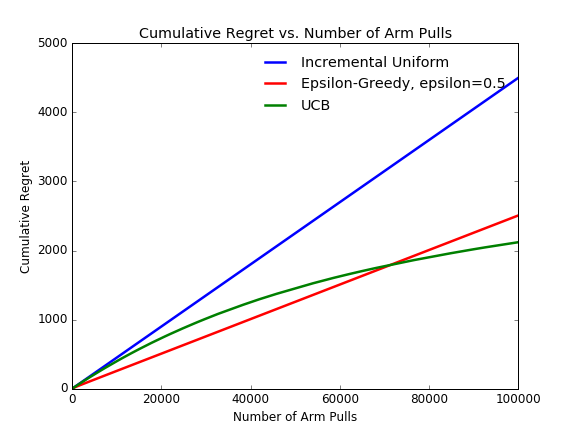
\includegraphics[width=1\linewidth]{bandit1_cumulative_regret.png}
\caption{Plot of cumulative regret for bandit 1 using different bandit algorithms. Note for UCB, the graph appears to be a logarithmic shape. If one keeps pulling more arms, the growth would slow down further.}
\label{fig:cumulative_bandit1}
\end{figure}

\begin{figure}
\centering
	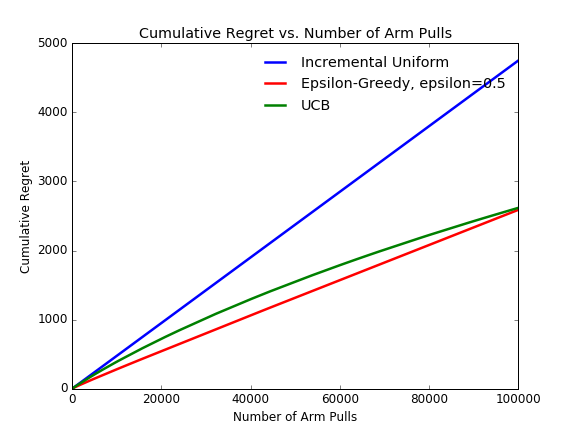
\includegraphics[width=1\linewidth]{bandit2_cumulative_regret.png}
\caption{Plot of cumulative regret for bandit 2 using different bandit algorithms. Note for UCB, the graph appears to be a logarithmic shape, though not as pronounced as for bandit1. One could keep pulling arms to confirm.}
\label{fig:cumulative_bandit2}
\end{figure}

\begin{figure}
\centering
	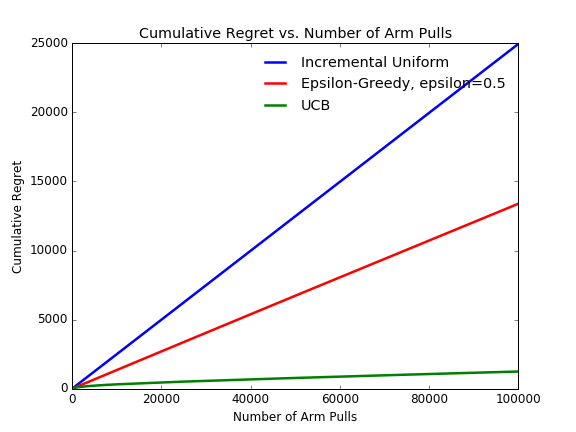
\includegraphics[width=1\linewidth]{custom_bandit_cumulative_regret.png}
\caption{Plot of cumulative regret for our custom bandit using different bandit algorithms.}
\label{fig:cumulative_bandit3}
\end{figure}

\subsection{Discussion}

The cumulative regret plots show that cumulative regret increases over time, which matches our expectations. Almost by definition, cumulative regret increases over time since at each time step it is accumulating the sum of regrets.

We also notice that for the UCB algorithm, the cumulative regret graph looks logarithmic. This also matches our expectation: looking at the theoretical bounds of the UCB algorithm, cumulative regret grows $O(\log n)$ where $n$ is the total number of arm pulls. UCB was also designed for the cumulative regret  objective so it is no surprise that it appears to be the best-performing algorithm out of the three bandit algorithms for optimizing cumulative regret.

\section{Part IV}

This section analyzes the simple regret of the bandit algorithms using the three different bandits from Part II. Simple regret is defined as $E[SReg_n] = R^{*} - E[R(a_{j_n})]$, where $R^{*}$ is the optimal expected reward (the maximum $p_a r_a$ out of all arms $a$) and $E[R(a_{j_n})]$ is the expected reward of the best arm that is being kept tracked by the algorithm, which in the case of SBRD bandits would be $p_a r_a$ where $a$ is the best arm kept tracked so far (the best arm does not necessarily mean the arm pulled at time $n$). Thus, simple regret is the difference between the optimal expected reward and expected reward of the best arm (selected by algorithm) at time $n$.

(Regrets are tracked and computed in regret.py. The plots are generated using plot.py.)

\subsection{Results}

Figures \ref{fig:simple_bandit1} and \ref{fig:simple_bandit1_zoomed} show the simple regret plot for bandit 1 using the bandit algorithms. Figures \ref{fig:simple_bandit2} and \ref{fig:simple_bandit2_zoomed} show the simple regret plot for bandit 2. Figures \ref{fig:simple_bandit3} and \ref{fig:simple_bandit3_zoomed} show the simple regret plot for our custom bandit.

We chose the number of trials to be $1,000$ to yield curves that were smooth enough. We chose number of arm pulls to be $100,000$, which is large enough to see the trend while not too large enough to take too much computation time. (We tried $1,000,000$ but it took too long with $1,000$ trials.)

Additionally, we can report which arm is the best as discovered by our algorithms. For bandit 1, the algorithm picks the best arm as the one with $r=1$ and $p = 0.1$. For bandit 2, the algorithm picks the 20th arm as the best arm ($r=1$ and $p = 0.1$). These match our expectations since they yield the optimal expected reward.

For reporting the best arm for bandit 3, table \ref{tab:arms} shows out of 1000 trials, the number of times each algorithm selected the $i$th arm as the best arm. We see that the last arm has the maximum number. Thus the algorithms were able to select the optimal arm as the best arm. However, it is still interesting to see that the algorithm ended picking the near-optimal arms as the best arm for quite a number of trials. It would be interesting to observe the numbers when the number of pulls is much greater.

\begin{table}
\begin{center}
\captionof{table}{Number of times algorithms selected the $i$th arm as the best arm} \label{tab:arms}
\begin{tabular}{ | l |c|c|c|c|c|c|c|c|c|c|c|c|c|c|c|c|c|c|c|c| }
  \hline
  Alg & 1 & 2 & 3 & 4 & 5 & 6 & 7 & 8 & 9 & 10 & 11 & 12 & 13 & 14 & 15 & 16 & 17 & 18 & 19 & 20\\ \hline
  IU & 0 & 0 & 0 & 0 & 0 & 0 & 0 & 0 & 0 & 0 & 60 & 59 & 50 & 67 & 61 & 56 & 68 & 63 & 56 & 460\\ \hline
  UCB & 0 & 0 & 0 & 0 & 0 & 0 & 0 & 0 & 0 & 0 & 23 & 30 & 30 & 30 & 31 & 28 & 28 & 29 & 24 & 747\\ \hline
  $\epsilon$-G & 0 & 0 & 0 & 0 & 0 & 0 & 0 & 0 & 0 & 0 & 32 & 37 & 32 & 40 & 37 & 34 & 31 & 35 & 29 & 693\\ \hline
\end{tabular}
\end{center}
\end{table}

\begin{figure}
\centering
	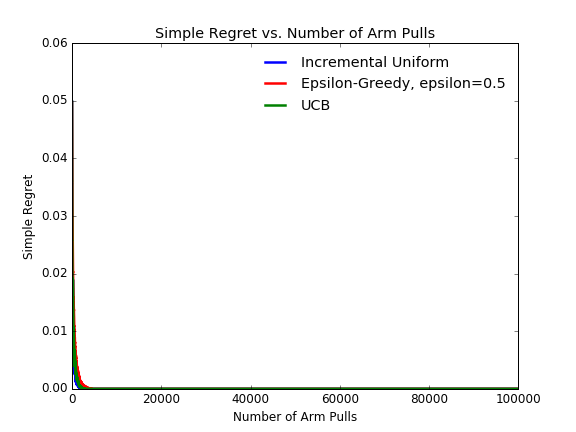
\includegraphics[width=1\linewidth]{bandit1_simple_regret.png}
\caption{Plot of simple regret for bandit 1 using different bandit algorithms.}
\label{fig:simple_bandit1}
\end{figure}

\begin{figure}
\centering
	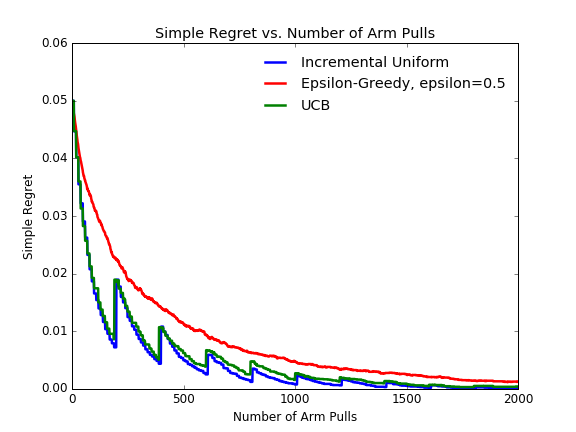
\includegraphics[width=1\linewidth]{bandit1_simple_regret_zoomed.png}
\caption{Plot of simple regret for bandit 1, zoomed in to visualize early behavior.}
\label{fig:simple_bandit1_zoomed}
\end{figure}

\begin{figure}
\centering
	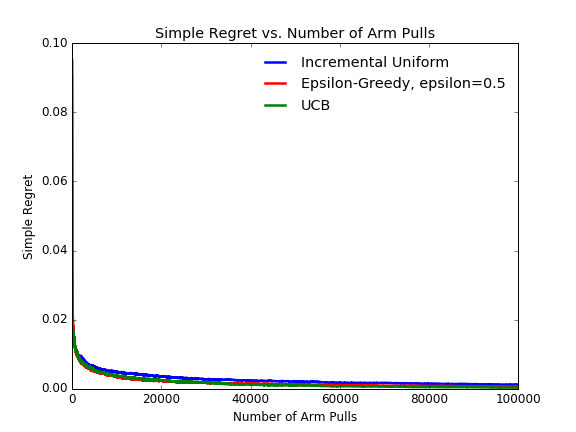
\includegraphics[width=.8\linewidth]{bandit2_simple_regret.png}
\caption{Plot of simple regret for bandit 2 using different bandit algorithms.}
\label{fig:simple_bandit2}
\end{figure}

\begin{figure}
\centering
	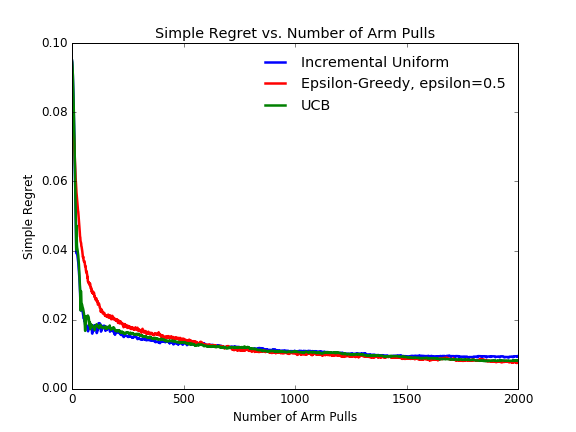
\includegraphics[width=1\linewidth]{bandit2_simple_regret_zoomed.png}
\caption{Plot of simple regret for bandit 2, zoomed in to visualize early behavior.}
\label{fig:simple_bandit2_zoomed}
\end{figure}

\begin{figure}
\centering
	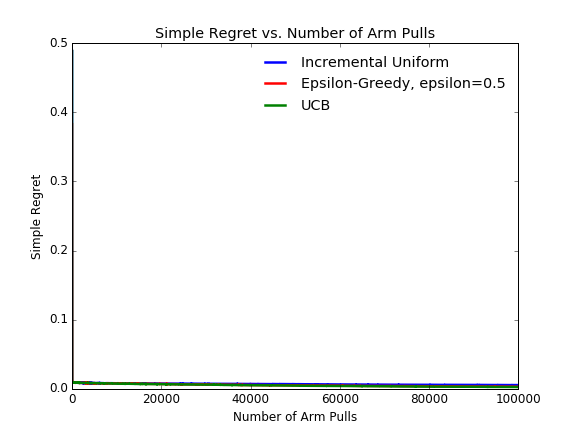
\includegraphics[width=.8\linewidth]{custom_bandit_simple_regret.png}
\caption{Plot of simple regret for our custom bandit using different bandit algorithms.}
\label{fig:simple_bandit3}
\end{figure}

\begin{figure}
\centering
	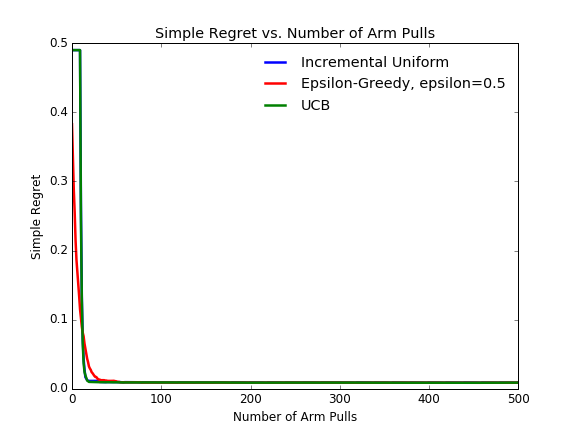
\includegraphics[width=1\linewidth]{custom_bandit_simple_regret_zoomed.png}
\caption{Plot of simple regret for bandit 3, zoomed in to visualize early behavior.}
\label{fig:simple_bandit3_zoomed}
\end{figure}

\subsection{Discussion}

The simple regret plots show that the simple regret is decreasing over time, which matches our expectations: simple regret does not accumulate sum of regrets over time but just looks at the difference between the optimal expected reward and the expected reward of the best arm selected by the algorithm.

What is surprising is that the plots suggest that $\epsilon$-greedy performs the worst (albeit the most stable) while incremental uniform and UCB perform roughly about the same but better than $\epsilon$-greedy. This empirical result does not match our expectations. We would expect UCB to reduce regret at a polynomial rate, incremental uniform to reduce at an exponential rate and $0.5$-greedy to reduce at a better exponential rate. Theory does not match practice sometimes.

For bandit 1, we also observe some ``periodic'' behavior in the graphs for incremental uniform and UCB. Perhaps this is because the algorithms are exploring consistently: it has to explore some bad arms sometimes in order to find the best arm to exploit in the end.

\end{document}